\documentclass[11pt,a4paper]{article}\usepackage[]{graphicx}\usepackage[]{color}
% maxwidth is the original width if it is less than linewidth
% otherwise use linewidth (to make sure the graphics do not exceed the margin)
\makeatletter
\def\maxwidth{ %
  \ifdim\Gin@nat@width>\linewidth
    \linewidth
  \else
    \Gin@nat@width
  \fi
}
\makeatother

\definecolor{fgcolor}{rgb}{0.345, 0.345, 0.345}
\newcommand{\hlnum}[1]{\textcolor[rgb]{0.686,0.059,0.569}{#1}}%
\newcommand{\hlstr}[1]{\textcolor[rgb]{0.192,0.494,0.8}{#1}}%
\newcommand{\hlcom}[1]{\textcolor[rgb]{0.678,0.584,0.686}{\textit{#1}}}%
\newcommand{\hlopt}[1]{\textcolor[rgb]{0,0,0}{#1}}%
\newcommand{\hlstd}[1]{\textcolor[rgb]{0.345,0.345,0.345}{#1}}%
\newcommand{\hlkwa}[1]{\textcolor[rgb]{0.161,0.373,0.58}{\textbf{#1}}}%
\newcommand{\hlkwb}[1]{\textcolor[rgb]{0.69,0.353,0.396}{#1}}%
\newcommand{\hlkwc}[1]{\textcolor[rgb]{0.333,0.667,0.333}{#1}}%
\newcommand{\hlkwd}[1]{\textcolor[rgb]{0.737,0.353,0.396}{\textbf{#1}}}%
\let\hlipl\hlkwb

\usepackage{framed}
\makeatletter
\newenvironment{kframe}{%
 \def\at@end@of@kframe{}%
 \ifinner\ifhmode%
  \def\at@end@of@kframe{\end{minipage}}%
  \begin{minipage}{\columnwidth}%
 \fi\fi%
 \def\FrameCommand##1{\hskip\@totalleftmargin \hskip-\fboxsep
 \colorbox{shadecolor}{##1}\hskip-\fboxsep
     % There is no \\@totalrightmargin, so:
     \hskip-\linewidth \hskip-\@totalleftmargin \hskip\columnwidth}%
 \MakeFramed {\advance\hsize-\width
   \@totalleftmargin\z@ \linewidth\hsize
   \@setminipage}}%
 {\par\unskip\endMakeFramed%
 \at@end@of@kframe}
\makeatother

\definecolor{shadecolor}{rgb}{.97, .97, .97}
\definecolor{messagecolor}{rgb}{0, 0, 0}
\definecolor{warningcolor}{rgb}{1, 0, 1}
\definecolor{errorcolor}{rgb}{1, 0, 0}
\newenvironment{knitrout}{}{} % an empty environment to be redefined in TeX

\usepackage{alltt}
\usepackage[top=1.00in, bottom=1.0in, left=1.1in, right=1.1in]{geometry}
\usepackage{graphicx}
\usepackage[numbers]{natbib}
\bibliographystyle{..//..//references/styles/nature.bst}

\usepackage[export]{adjustbox}
\IfFileExists{upquote.sty}{\usepackage{upquote}}{}
\begin{document}


\includegraphics[width=0.2\textwidth, right]{AA_logo.jpg}
\noindent 1300 Centre Street\\
\noindent Boston, MA, 20131\\

\vspace{1.5ex}

\pagenumbering{gobble}

\noindent{Dear Dr. Hetherington:}
\vspace{3ex}\\
\noindent Please consider our manuscript, `False springs coupled with warming winters alter temperate tree growth', as a Full Paper for \textit{New Phytologist}. \\

\noindent Biological spring is advancing with climate change but late spring freeze dates are not predicted to advance at the same rate, leading to renewed interest in late spring freeze events---commonly called `false springs'---which shape the life history of many temperate and boreal plant species. At the same time over-winter chilling may decrease with warming winters, which could impact plant phenology and, ultimately, growth. Together, false springs and warmer winters could reshape forest plant communities, with cascading effects on pollinators, nutrient cycling and carbon uptake.  \\ % Let's say why this is important early!

\noindent \textit{What hypotheses or questions does this work address?} With recent climate change, there is growing interest in false springs and decreasing over-winter chilling, which---combined---could reshape forest plant communities. We assess the effects of false springs and decreased chilling on sapling phenology, growth and tissue traits, across eight temperate tree and shrub species in a lab experiment. \\

\noindent \textit{How does this work advance our current understanding of plant science?} We found that false springs increased tissue damage, decreased leaf toughness and leaf thickness, and slowed budburst to leafout timing---extending the period of maximum freezing risk. Decreased over-winter chilling further increased this period of maximum risk, thus increasing the detrimental effects of false springs. Our findings disentangle how winter chilling and spring freeze events shape tree growth across species, and suggest climate change could deminish or reverse carbon storage in temperate forests. Further, our focus on interactive effects of warmer winters and springs applies widely to a diversity of plant taxa. \\

\noindent \textit{Why is this work important and timely?} For over a decade, increasing evidence has suggested false springs are shifting with climate change and in turn reshaping forest dynamics. Yet studies of direct impacts of false springs on phenology and growth, especially across species, has been limited because most studies are observational and often rely on satellite metrics such as 'green-up.' We present the first lab experiment to document the effects of false springs and combine it with chilling to understand the interplay of these two factors---across eight tree species. Our findings of how false spring and chilling alter phenology, growth and tissue investment have implications for models of forest plant communities, future carbon storage and climate change itself. \\

\noindent This manuscript is not under consideration elsewhere. Both authors approved of this version for submission. We hope that you will find it suitable for publication in \textit{New Phytologist}. Thank you for your consideration. \\

\vspace{1.5ex}
\noindent Sincerely, \\
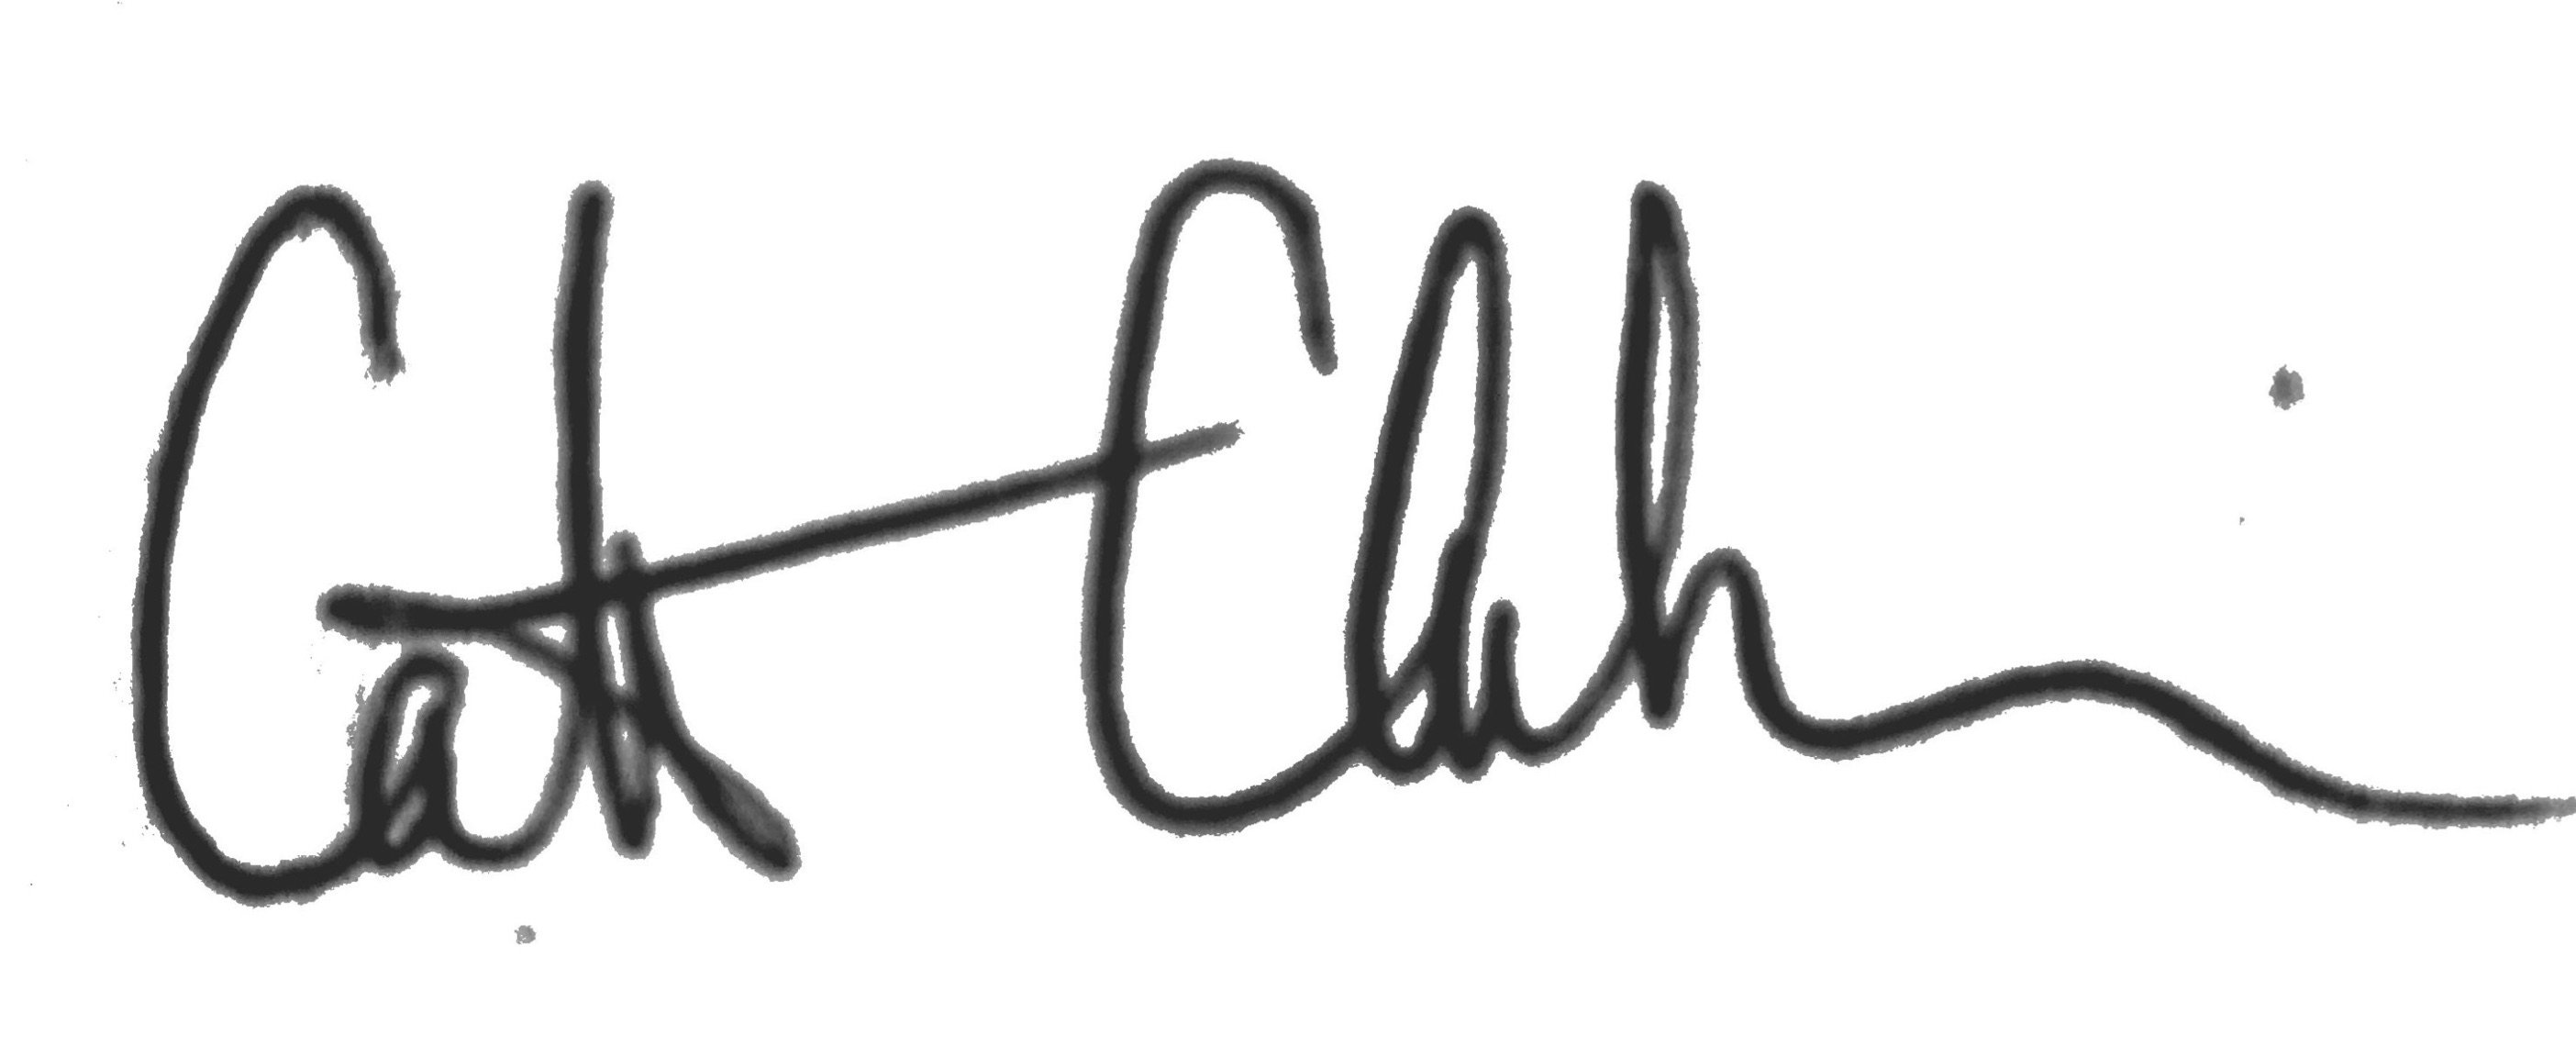
\includegraphics[width=0.2\textwidth]{full_signature.jpg} \\
\noindent Catherine Chamberlain (on behalf of my co-author)
\vspace{2ex}\\
\noindent Authors:\\
C. J. Chamberlain $^{1,2}$ \& E. M. Wolkovich $^{1,2,3}$
\vspace{2ex}\\
\emph{Author affiliations:}\\
$^{1}$Arnold Arboretum of Harvard University, 1300 Centre Street, Boston, Massachusetts, USA; \\
$^{2}$Organismic \& Evolutionary Biology, Harvard University, 26 Oxford Street, Cambridge, Massachusetts, USA; \\
$^{3}$Forest \& Conservation Sciences, Faculty of Forestry, University of British Columbia, 2424 Main Mall, Vancouver, BC V6T 1Z4\\
\vspace{2ex}
$^*$Corresponding author: 248.953.0189; cchamberlain@g.harvard.edu\\

%\bibliography{..//..//references/chillfreeze.bib}

\end{document}
